\graphicspath{{./design/}}

\chapter{Design}
% {{{
\label{cha:Design}

% {{{

A very modular approach to the design of the system was taken. A number of
required components was identified and categorised. The main component
categories of the system are:

\begin{itemize}
  \item Simulation I/O - handles input and output of data
  \item Coders - encodes and decodes symbols
  \item Compressors - drivers behind the compression
  \item Visualisation - displays the simulation data
  \item General components - general transformations
  \item Method specific components - components specific to a particular
  compression scheme
  \item Verification components - verify and record various aspects of the
  system
\end{itemize}

A brief overview of the different components and how they are used is provided
for in Section \ref{sec:design_overview}, while Section
\ref{sec:design_visualisation} will provide more detail into the
visualisation components of the system.

% }}}

\section{System overview}
% {{{
\label{sec:design_overview}

The executables of the system are within the Compressors and Visualisation
component categories, there are multiple executables so that
compression/decompression does not require a GUI being available.

The compression program (within Compressors or Visualisation), will use the
Simulation I/O components to read the molecular data, which will then be
transformed using the General components, the output of which will be used by
the Coders and Visualisation components. The Coders may have their own specific
components (Method specific components), which will be used to perform the
encoding/decoding of symbols. The Verification component will connect to the
various other components that it is measuring.

See figure TODO for a schematic diagram of all the components of the system,
and how they relate to each other.

% TODO: add diagram of components, and how they link up
[provide a schematic diagram of all the components and how they link up].

% }}}

\section{Visualisation}
% {{{
\label{sec:design_visualisation}

% {{{

With regards to the visualisation category, there are a number of components
within it, each of which will be responsible for presenting the molecular data
in a different manner.

\begin{itemize}
  \item Water point rendering
  \item Metaballs rendering
  \item Water cluster visualisation
  \item Quantisation error visualisation
\end{itemize}

% }}}

\subsection{Water point rendering}
% {{{
\label{sub:design_waterpoint}

This rendering technique is the simplest of all the visualisation techniques in
the system. A very transparent point will be drawn for each of the water
molecules. The points will be almost transparent so that a sense of the size
and depth of the volume can be seen; the colour at a particular point will
become more pronounced as more water molecules overlap there. See figure
\ref{fig:design_waterpoint}.

The advantage of this rendering technique is that it easily identifies and
highlights the larger bodies of water in the molecular data. The non-water
molecules has been filtered out so as to avoid obscuring the water molecules.

\begin{figure}[h!]
  \begin{center}
    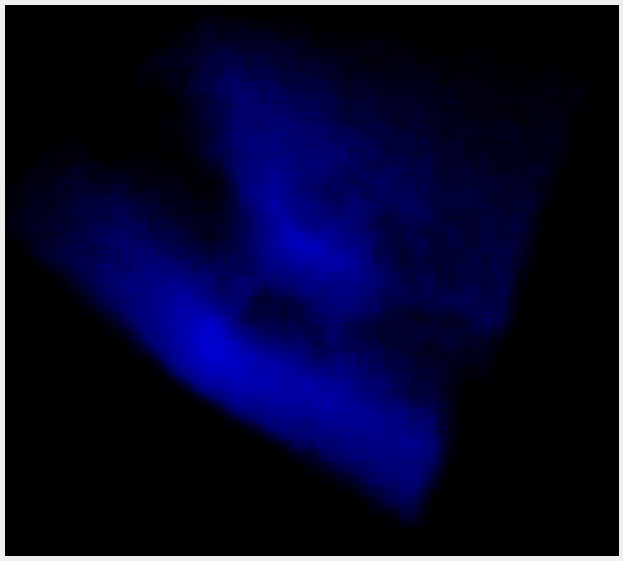
\includegraphics[width=70mm]{waterpoint}
  \end{center}
  \caption{Water point rendering, each point represents a water molecule}
  \label{fig:design_waterpoint}
\end{figure}

% }}}

\subsection{Metaballs rendering}
% {{{
\label{sub:design_metaballs}

The metaballs technique (Section \ref{sub:background_metaballs}) was chosen as
an alternative way to visualise the water volume in the molecular simulation as
it will group the water molecules together, hence providing some clutter
reduction. See figure TODO. The boundary of the water volume can be clearly
seen with metaballs, with water point rendering the boundary is not as clearly
visible.

% TODO: implement and compare marching tetrahedrons and marching cubes
[TODO: implement marching cubes, compare to marching tetrahedra, say which was
chosen as final implementation and why]

To determine the surface of the volume, the marching tetrahedrons algorithm was
used. Marching tetrahedrons was chosen over marching cubes for surface
extraction as it was easier to implement due to there is no ambiguity handling,
nor are lookup tables needed for the algorithm.

As the molecular data will need to be explored and displayed in real time, the
mesh obtained from the surface extraction will need to be simplified. This can
be accomplished by either increasing the grid size when sampling the volume to
determine the surface, or by mesh decimation. As mesh decimation provides more
control over what the final surface will look like, a mesh decimation algorithm
has been implemented.

Mesh decimation will be accomplished using the vertex clustering approach.
Vertex clustering was used instead of geometric decimation as it is more
computationally efficient and it integrates well with the surface extraction
part of the rendering process.

[TODO: implement another decimation approach to see what the speed differences
are?]

[TODO: maybe be able to control the near viewing plane so that you get a
'slice' of the volume? Otherwise occlusion of the stuff behind will happen?]

[TODO: insert final image]

% }}}

\subsection{Water cluster visualisation}
% {{{
\label{sub:design_watercluster}

The water molecules in a body of water is not completely uniform in all
directions, instead the water molecules form clusters. To visualise these water
clusters, a ribbon will be used to connect and show these clusters. This is
be similar to the ribbon model for protens (\citep{richardson81},
\citep{carson87}) and the twister visualisation technique \citep{kuttel06}.

Using a ribbon to connect the water molecules within the cluster allows for
clusters to be easily identified, as well as the orientation of the cluster.
See figure TODO for an image of a single water cluster.

To cope with the large number of water clusters that will be present, a level
of detail scheme has been implemented. The user is able to zoom in and focus on
a specific area of the volume, all the water clusters outside of this area has
been faded out so as to provide context, but not clutter the display.  The user
is also able to focus on and follow a specific water cluster. See figure TODO
for an image where an area has been focused on.

[TODO: insert final image]

% }}}

\subsection{Quantisation error visualisation}
% {{{
\label{sub:design_quanterror}

This component is not strictly a visualisation component, but is more a
verification component that visually displays some data.

Quantisation is the only lossy step of the compression, thus it is important to
measure the amount of error that is introduced. To visually depict the
quantisation errors, the water molecules are coloured according to a colour
gradient. Water molecules with high quantisation errors are coloured so that
they are more visible and stand out. See figure TODO to see a quantisation
error image.

[TODO: insert final image]

% }}}

% }}}

% }}}

% {{{

\newpage
\section{My questions (NOT TO BE INCLUDED IN FINAL REPORT)}

\begin{enumerate}

  \item
  I know that the tense of this chapter is quite confused. It has to do
  with the way that I was thinking when I typed this up (some of the stuff
  hasn't been implmented yet). I'm assuming that this chapter should phrase
  things in the past and present tense? i.e. the system \emph{currently} does
  this and this because these \emph{were} the tradeoffs\dots

  \item
  I imagine that this chapter may change or be rephrased as the implementation
  progresses. I hope to be able to do all the things I've identified, but if
  not then some pruning will need to happen. I seem to have a habit of going
  above and beyond what I set out initially to do\dots

  \item
  How much detail should we go into for the design chapter? I couldn't find
  much to say without going into implementation details.  As was mentioned, the
  design chapter shouldn't be a list and description of all the components, but
  all the components are very straight forward and relatively simple,
  especially for the visualisation...

  \item
  How much of this chapter will overlap with the implementation chapter?
  That is assuming that there will be an implementation chapter? Or should
  implementation be merged into this chapter, i.e. a "Design and
  Implementation" chapter?

\end{enumerate}

% }}}
